\documentclass[a4paper, 11pt]{article}
\usepackage[english]{babel}
\usepackage[ansinew]{inputenc}
\usepackage{graphicx}
\pagestyle{headings}

\begin{document}
\bibliographystyle{alphadin}

\title{Detection of Nucleoli Using ImageJ}
\author{Nico Hochberger}
\date{November 2014}
\maketitle

\newpage
\tableofcontents

\newpage
\section{Introduction}

\subsection{Preface}
 
\subsection{Objective}

\subsection{Motivation}
Currently nucleoli are detected using an application called
CellProfiler\footnote{http://www.cellprofiler.org}.
While this application yields reliable results, it also takes pretty long to complete
the analysis. Runtimes up to 45 seconds are common.
Due to the fact that CellProfiler is a very general approach, applicable to a
large variety of tasks related to detecting nuclei and nucleoli, the results of
its analysis have to be checked manually to reduce the amount of
false-positives.
In order to analyze the cells, they need to be taken out of the incubator. Yet,
outside the incubator the cells can only be kept alive for a limited timespan.
Considering this, time is a valuable resource and must not be wasted by using a
too general approach.
Consequently, this leads to a more specialized way of analyzing the cells, which
does not do all the analysis performed by CellProfiler, but on the other hand is
much faster and thus helps to prevent cells dying before the analysis is
finished.
\begin{figure}[h]
    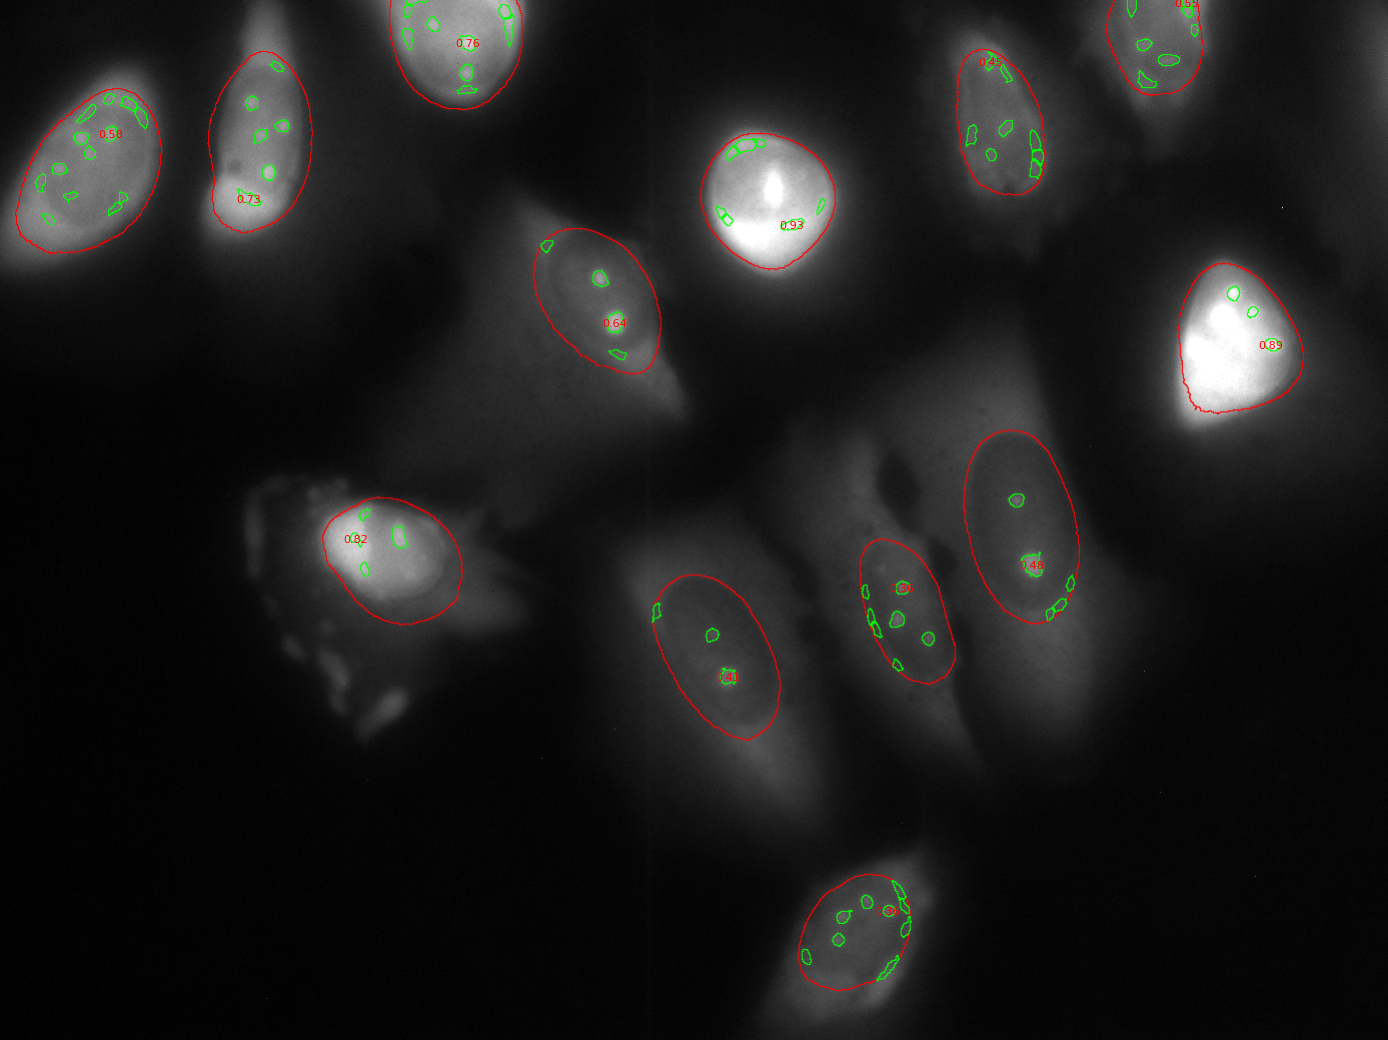
\includegraphics[width=\linewidth]{images/cellprofiler_channel1}
    \caption{Example analysis performed with CellProfiler}
    \label{fig:cellprofiler_example}
\end{figure}

\newpage
\section{Design and Implementation}

\subsection{Requirements}

\newpage
\section{User's Manual}

\subsection{System Requirements}

\subsection{Starting the Application}

\subsection{Configuration}
\subsubsection{General Parameters}
\subsubsection{Improved Image Detection Parameters}
\subsubsection{Structure of Files and Folders}

\newpage
\section{Conclusion and Prospect}
 
\subsection{Conclusion}

\subsection{Prospect}


\newpage
\addcontentsline{toc}{section}{Bibliography}
\bibliography{sources}

\end{document}